\documentclass[12pt, a4paper, twoside]{article}

\usepackage[dutch]{babel}
\usepackage{graphicx}
\usepackage{url}
\usepackage{graphicx}
\usepackage{multicol}
\usepackage[pdftex]{bookmark}

\newcommand{\casam}{C.A.S.A.M. }
\newcommand{\casamproject}{C.A.S.A.M.-pro\-ject }
\hyphenpenalty=10000
\sloppy

%\setlength{\oddsidemargin}{100pt}
%\setlength{\evensidemargin}{100pt}
%\setlength{\marginparwidth}{57pt}
%\setlength{\footskip}{30pt}

\title{\casamproject Eindverslag}
%\subtitle{Bachelor project IN3405}
\author{S.E.F. van Berkel (1262882) \and B. Bijl (1312405)\and J.Y.T. den Hollander (1268538)\and S. Rabbelier (1308211)\and B.M.W. Sedee (1263153)\and N.N. Smit (1286455)}

\begin{document}

\begin{titlepage}

\maketitle

\thispagestyle{empty}

\begin{center}
\vspace{2cm}
\large
Opdrachtgever: Erasmus Medisch Centrum \\
Begeleiding: Technische Universiteit Delft\\
Faculteit Elektrotechniek, Wiskunde en Informatica\\

\vspace{5cm}
Beoordelingscommissie: \\
Dr. C.P. Botha \\
Dr. G.J. Kleinrensink \\
Ir. M. Sepers

\end{center}

\end{titlepage}
\pagenumbering{alph}
\newpage
\thispagestyle{empty}
\mbox{}
\newpage
\thispagestyle{empty}
\begin{quote}
\begin{center}

\emph{
All models are wrong, but some are useful
\\ -George E.P. Box
}
\end{center}
\end{quote}
\medskip
\begin{quote}
\begin{center}
\emph{
Perceive those things which cannot be seen
\\ -Miyamoto Musashi
}
\end{center}
\end{quote}
\medskip
\begin{quote}
\begin{center}
\emph{
Javascript: It is a dark festival of pain
\\ -http://www.wooji-juice.com/blog/javascript-article.html
}
\end{center}
\end{quote}
\newpage

\setcounter{tocdepth}{3}

\pagenumbering{roman}
\setcounter{page}{1}
\tableofcontents

\newpage
\noindent
\pagenumbering{arabic}
\setcounter{page}{2}

%\addcontentsline{toc}{section}{Voorwoord}

\section{C.A.S.A.M. werking door samenwerking.}
In 2008 begon Anton Kerver met zijn afstudeeropdracht: het in kaart brengen van een gebied waar veilig ('safe zone') een laserbehandeling voor spataderen kan plaatsvinden.
\\
\\
Al snel kwam de vraag: hoe kunnen wij de enorme hoeveelheid data bruikbaar (lees: visueel) maken  voor de gebruiker, de (in dit geval) vaatchirurg. Toen Anton op het Internet ging surfen om een manier te vinden van datavisualisatie kwam hij terecht bij commercieel beschikbare 'Morphing' programma's. Hij wist, als (op de medische faculteit) erkende whizzkid snel de principes te doorgronden van het programma en ging vrolijk aan de slag�prachtige platen en echt prachig in beeld gebrachte safe zones waren het gevolg�alle problemen opgelost�klaar is Kees.
\\
\\
�..totdat de vragen gecompliceerder werden�HOE worden de beelden gemorpht, welke mate van precisie wordt gehanteerd, hoe krijgen we het systeem beschikbaar, hoe kan de individuele chirurg (en dus de pati\"{e}nt) tijdens een operatie profiteren van deze data�enfin Kees was helemaal niet klaar�.
Historisch gezien ging het bij ons op de afd. Neuroscience-Anatomie altijd zo: onoplosbaar technisch probleem? Delft bellen�en wel onmiddellijk! Instant succes volgt dan weliswaar niet maar meestal binnen een maandje of twee is er het verlossende woord uit Delft.
\\
\\
Zo ook nu dus. Om een lang verhaal kort te maken�na een zoektocht door de verschillende faculteiten en afdelingen van de TU Delft kwamen we terecht bij Charl Botha en Frits Post v.d. fac. Electrical Engineering, Mathematics and Computerscience,  afd. Medical Visualisation. Precies raak: enthousiaste mensen die ons gelijk op ons gemak stelden�neen, wij hadden geen onwezenlijke wensen en ja, zij konden ons zeker helpen. Charl, heeft na een collegecyclus over het onderwerp medische data-visualisatie een oproep gedaan onder zijn studenten om een bachelorproject te doen met onze vraagstelling als uitgangspunt.
\\
\\
Binnen 3 weken was daar onze groep studenten�.6 enthousiastelingen die stonden te popelen om ons te helpen�.de IT termen vlogen over de tafel en na een kwartier werd het duidelijk�wij medici begrepen totaal niet waar ze het over hadden en zij wisten in het geheel niet wat wij wilden, maar�� dit wordt mooi! En mooi werd het. Bastiaan Bijl, Ben Sedee, Jaap den Hollander, Noeska Smit, Sjors van Berkel en Sverre Rabbelier gingen aan de slag, hadden veel contact met Anton en tussentijds vielen onze monden al open, maar wat er na een, toch beperkte tijd, van 10 weken nu voor ons ligt overtreft onze stoutste verwachtingen. 
\\
\\
Wat vooral opviel was de unieke samenkomst van talenten: ieder lid van de groep had zijn eigen specialisme (van communicatie met de leek tot wiskundige expertise tot effectief project management) en niet alleen brachten zij hun eigen kennis in�de anderen hadden de positief-actieve instelling om zich deze kennis eigen te maken. Een echte zelflerende groep met respect voor elkaars identiteit. Met als resultaat: een fantastische oplossing voor ons probleem en een geweldige basis voor uitbreiding naar een web-based consultatiesysteem voor chirurgen met direct positieve effecten voor de (chirurgische)pati\"{e}nt! Met dit programma kunnen we jarenlang vooruit�alle chirurgische toegangen tot het menselijk lichaam kunnen nu op een gefundeerde wijze, compleet met statistische onderbouwing worden bestudeerd en ter beschikking worden gesteld, waarmee de Computer Assisted Surgical Anatomy Mapping (C.A.S.A.M.) droom werkelijkheid kan worden. Bastiaan, Ben, Jaap, Noeska, Sjors en Sverre heel veel dank voor jullie enthousiasme en inzet en voor de ervaring hoe een groep gemotiveerde specialisten tot grote hoogte kunnen komen door onzelfzuchtige, echte samenwerking. 
\\
\\
Onze Hartelijke dank!
\\
\\
Dr. Gert-Jan Kleinrensink
\\
Drs. Anton Kerver

\newpage
%\setcounter{section}{-1}
\section{Samenvatting}

Met het \casamproject is er tien weken lang gewerkt door zes Bachelor studenten van de TU Delft aan een systeem dat het \casamproject op het Erasums Medisch Centrum faciliteert. 
In dit ziekenhuis is Anton Kerver bezig meerdere preparaten te maken om voor bepaalde chirurgische ingrepen visueel te kunnen tonen hoe een gemiddelde pati\"{e}nt in elkaar zit.

Het systeem dat ontworpen is biedt een databasestructuur met een browser-interface waarin foto's van preparaten behorend tot \'{e}\'{e}n ingreep als project gegroepeerd opgeslagen worden. 
Vervolgens kunnen er per foto landmarks aangegeven worden en kunnen belangrijke gebieden overgetekend worden.
Ook is het mogelijk om meerdere foto's zichtbaar te maken, in combinatie met de landmarks en bitmaps die bij deze foto's horen.
Deze landmarks en bitmaps kunnen vervolgens ook eventueel onzichtbaar gemaakt worden.
Een gemaakte compositie van zichtbare foto's, landmarks en bitmaps kan opgeslagen worden als state, zodat deze later weer makkelijk op te vragen is.

Als op meerdere foto's dezelfde landmarks zijn aangegeven, is het mogelijk om visueel de variatie te tonen binnen de landmarks met behulp van een Point Distribution Model. 
Op deze manier kunnen verschillen tussen foto's gemakkelijk inzichtelijk gemaakt worden.
Een tweede toepassing van Image Processing is de mogelijkheid om verschillende bitmaps met elkaar te morphen. 
Dit houdt in dat de verschillende bitmaps zodanig vervormd en verplaatst worden, dat ze allemaal op hetzelfde been van toepassing zijn, zodat de variaties tussen bepaalde gebieden op verschillende foto's zichtbaar gemaakt kan worden.

Het is verder mogelijk om papers en weblinks aan projecten te koppelen.
Hiernaast is het systeem voorzien van een aantal hulpfuncties zoals een zoomscherm en de mogelijkheid om gedane acties ongedaan te maken. 

Bij met maken van het systeem is gebruik gemaakt van een Django framework dat met Python werkt en webpagina's genereerd die op de client een JavaScript-applicatie draait. 
Ook is er voor \'{e}\'{e}n functie een Flash-applicatie geschreven.
Deze samensmelting van verschillende technologi\"{e}n was voor onze groep een volledig nieuwe ervaring, die ons uiteindelijk goed is bevallen.

\newpage
\section{Inleiding}
\label{inleiding}
De afgelopen tien weken hebben wij met elkaar gewerkt aan een webapplicatie voor het \casamproject. Voor het vervullen van deze opdracht hebben wij op diverse terreinen verschillende uitdagingen moeten overwinnen. Dit ging van de communicatie met experts van het Erasmus Medisch Centrum die geen verstand hadden van de IT-wereld, tot aan het werken met programmeertalen waar niemand ervaring mee had. 
Uiteindelijk hebben we een product gebouwd dat vele verschillende programmeertalen bij elkaar brengt en op deze manier gebruiken we de verschillende krachten in een nieuwe combinatie. Ook hebben wij het idee dat het product voldoet aan de eisen van het \casamproject. Dit resultaat hebben wij ook te danken aan het Agile programmeerprincipe waardoor wij veel tussentijds contact hebben gehad met de opdrachtgever en de uiteindelijke gebruikers.
\\
\\
In dit verslag besteden wij aandacht aan de verschillende uitdagingen die voor ons lagen, de oplossingen die we daarvoor hebben gevonden en het research wat we daarvoor hebben moeten doen. In sectie 2 leggen we uit wat de probleemstelling is en daaraan gekoppeld wordt in sectie 3 een analyse gemaakt van het probleem en een oplossingsrichting gedefinieerd. In sectie 4 zullen we ingaan op de planning die we hebben gemaakt, om in sectie 5 in te gaan op de aanpak van ons probleem. Daarna zullen we in sectie 6 een toelichting geven op onze implementatie en een aantal bijzondere aspecten uitlichten. Om daarna in sectie 7 een analyse te maken over de mogelijkheden om het product uit te breiden en te verbeteren. 
\\
\\
Bij dit verslag horen enkele document welke zijn toegevoegd als bijlage. Voorbeelden hiervan zijn het Plan van Aanpak, het orientatieverslag en het RAD-document van de database applicatie. In het verslag zal op verschillende momenten worden verwezen naar deze documenten. 

\newpage
\section{Probleemstelling en Analyse}
\label{Probleemstelling_en_analyse}
\subsection{Probleemstelling}
Het \casamproject was op zoek naar een applicatie die hun kon helpen bij de anatomische vraagstukken die zij hadden. 
Het ging hierbij vooral om hulp bij het morphen van foto's en de mogelijkheden om op verschillende foto's bijzonderheden aan te kunnen geven en deze met elkaar te vergelijken. 
Al in het eerste gesprek bleek dat er op dat moment nog geen enkele applicatie lag en dat alle foto's gewoon werden opgeslagen op een harde schijf en dat er out-of-the-box software werd gebruikt voor de foto manipulatie. 
Op dat moment hebben wij voorgesteld om naast de foto manipulatie ook aandacht te besteden aan de administratie en opslag van het materiaal.
Tenslotte kwamen zij ook met de vraag of het mogelijk was om bepaald materiaal dat in het ziekenhuis werd gemaakt, zoals r\"{o}ntgenfoto's, direct te importeren in het systeem. Ook wilde zij graag publicaties die hoorde bij een project erbij opslaan.

\subsection{Analyse}
In overleg met de C.A.S.A.M.-projectgroep hebben we toen afgesproken om het project in drie delen op te delen: de database-applicatie, Image processing en tenslotte de koppeling met andere systemen. 
Daarnaast werd meteen afgesproken dat de projectgroep op de TU Delft zou werken, dit omdat de facilitaire mogelijkheden in Delft beter zijn dan op het Erasmus MC. 
Om wel voldoende feedback te blijven ontvangen is er gekozen voor een Agile programmeerprincipe, op deze manier zou de opdrachtgever voldoende betrokken blijven bij het proces.
\\
\\
In de eerste week van het project hebben wij een lijst opgesteld van de verschillende functionaliteiten die in het systeem moesten komen. 
Van te voren was al duidelijk dat niet alle functionaliteiten gebouwd konden worden binnen de scope van dit project. 
Daarom zijn in samenspraak met de opdrachtgever de functionaliteiten van prioriteiten voorzien, uiteindelijk is daar een diagram uitgekomen, zie hiervoor bijlage A.
\\
\\
Mede op basis van het prioriteiten diagram hebben wij de verschillende uitdagingen gedefinieerd:
\begin{itemize}
  \item Project gerelateerd
  \begin{itemize}
    \item Gebrek aan medische en anatomie kennis
    \item Gebrek van IT kennis aan de kant van de opdrachtgever
    \item Samenwerking in een grote groep
  \end{itemize}
  \item Database systeem
  \begin{itemize}
    \item Gebruikersvriendelijkheid
    \item Van diverse locaties bereikbaar
    \item Eenvoudige manier om data toe te voegen aan het systeem
    \item Schaalbaarheid
  \end{itemize}
  \item Image processing
  \begin{itemize}
    \item Variaties in landmarks weergeven
    \item Morphen van verschillende foto's naar \'{e}\'{e}n gemiddelde foto
    \item Verplaatsen en roteren van foto's naar standaard view
  \end{itemize}
\end{itemize}
In de volgende secties lichten wij toe hoe we met deze uitdagingen zijn omgegaan.

\newpage
\chapter{Planning}
\label{Planning}
We begonnen het project met het maken van een planning voor de komende tien
weken zodat het voor zowel de opdrachtgever als onszelf duidelijk was wanneer
er wat gedaan zou worden. In verband met de Agile methoden zijn de eerste paar
weken meer in detail gepland dan de latere weken met de bedoeling om de
planning steeds bij te werken voor de komende (paar) weken. Deze voorgenomen
planning wordt besproken in paragraaf \ref{voorgenomen_planning}. Voor een
uitgebreidere beschrijving van de diverse fasen zie het Plan van Aanpak.
Zoals verwacht is deze ruwe planning aangepast in de
weken daarna, deze realisatie wordt besproken in \ref{werkelijke_planning}.

\section{Voorgenomen planning}
\label{voorgenomen_planning}
Doordat we in het begin slechts een grove planning hadden gemaakt, waren vooral
de eerste paar weken in detail uitgewerkt.
Er moesten twee documenten af zijn voordat er met de implementatie van het product kon worden begonnen, dit zijn het Plan van Aanpak en het Requirement Analysis Document.
Tevens hebben we ons direct voorgenomen een demo in de eerste weken van het project te maken zodat de opdrachtgever snel feedback kon geven op de richting waar het project in gaat.
Aangezien de tentamens op 16 juni beginnen, is afgesproken voor deze datum het project af te ronden.
In de onderstaande Ganntchart wordt de planning zichtbaar gemaakt zoals wij het aan het begin van het project voorstelden:
\\
\\
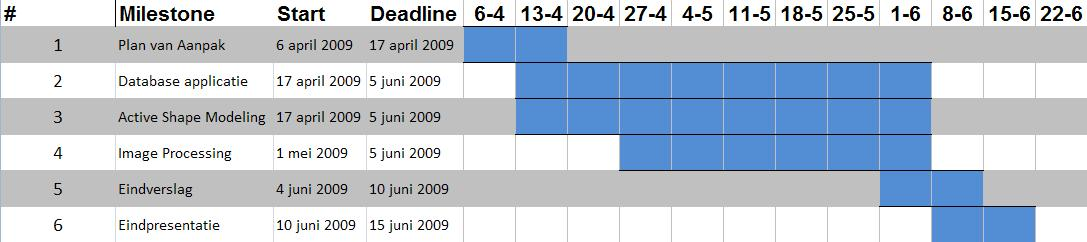
\includegraphics[width=0.9\textwidth]{ganntbefore}

\subsection{Plan van Aanpak}
Tijdens ons eerste gezamelijk overleg is het volgende schema voor het PvA
afgesproken, waarbij de deadlines zijn vastgesteld met de gelegenheid in het achterhoofd om verbeteringen later door te voeren.

\noindent 09 april: Concept PvA mailen \\
14 april: Verwerken feedback PvA \\
15 april: Meeting in erasmus \\
17 april: PvA af

\subsection{Requirement Analysis Document}
Voor het RAD is een (minder granulaire) planning gemaakt. Deze overlapt
de planning voor het PvA. Het schrijven van het tweede document en
het verwerken van verbeteringen aan een ander document kunnen tegelijk worden
uitgevoerd.
\\
\\
Nadat de tweede ronde van feedback op het PvA was verwerkt werd begonnen met
het RAD, zodat deze zo snel mogelijk afgerond kon worden en aan de
implementatie kon worden begonnen. Eventuele feedback op het PvA hierna werd
eerst verwerkt.

\noindent 27 april: RAD af

\subsection{Database Applicatie}
Om een demo te kunnen geven waarna zo veel mogelijk ge\"{e}valueerd kan worden
over de gewenste functionaliteiten was besloten om de twee weken na het
inleveren van het RAD te besteden aan het maken van spike solutions en deze te
integreren in een simpele applicatie die de basisfunctionaliteiten aan de
opdrachtgever presenteert.

\noindent 08 april: Database Applicatie af

\subsection{Active Shape Modelling}
Een belangrijk deel van de applicatie is het weergeven van de hoofdmodi van
variatie per landmark type en het weergeven van de gemiddelde landmarks.

\noindent 25 april: Active Shape Modelling af

\subsection{Image Processing}
Aanvankelijk zagen we deze fase als het projecteren van resultaten op
bijvoorbeeld r\"{o}ntgenfoto's. In de loop van het project hebben we de
betekenis van deze fase echter veranderd in het tekenen van gebieden en
morphen van deze gebieden naar een gemiddeld been. Dit is een cruciale fase
voor de aangeboden oplossing.

\noindent 11 april: Image Processing af

\subsection{Eindverslag}
Het schrijven van het eindverslag moet ruim voor de eindpresentatie afgerond
zijn zodat het verslag goedgekeurd kan worden voor aanvang van de eindpresentatie.

\noindent 12 april: Eindverslag af

\subsection{Eindpresentatie}
De eindpresentatie is de uiteindelijke afronding van het project.

\noindent 19 april: Eindpresentatie gegeven

\section{Werkelijke planning}
\label{werkelijke_planning}
In deze sectie geven wij aan hoe de opgestelde planning aansluit op de
uiteindelijke realisatie.
\\
\\
Zowel het PvA als het RAD waren op tijd af. De andere milestones zijn
gewijzigd. Omdat verschillende leden van de projectgroep tentamens
hebben in de weken vanaf 15 juni is besloten om het project rond deze datum af
te ronden. Hierdoor schoven de deadlines voor het schrijven van het eindverslag
en het geven van de eindpresentatie naar voren op.
\\
\\
In de originele planning is hierdoor de deadline het eindverslag naar 10 juni verschoven en zal de eindpresentatie op 15 juni plaatsvinden.
Door een goede scheiding van de verschillende functionaliteiten bleek het goed mogelijk om een werkverdeling te maken waar iedereen zijn of haar expertisegebieden in kwijt kon.
Hierdoor liepen de Database Applicatie, Active Shape Model en Image Processing fasen parallel aan elkaar en werden de laatste werkzaamheden tegelijk afgerond.
\\
\\
In de latere weken van het project bleek ook nog enige tijd nodig om de code te
refactoren, bugs te verwijderen en functionaliteiten verder te verbeteren. Dit
zorgde ervoor dat de eerdergenoemde drie parallel lopende fasen wat uitliepen.
\\
\\
In de originele planning was geen rekening gehouden met de tijd die nodig is om
de applicatie ook te laten draaien op een server in het Erasmus MC. Hierdoor
vindt dit tegelijk plaats met het schrijven van het verslag.
In de onderstaande Ganntchart is te zien hoe de werkelijke planning verliep:
\\
\\
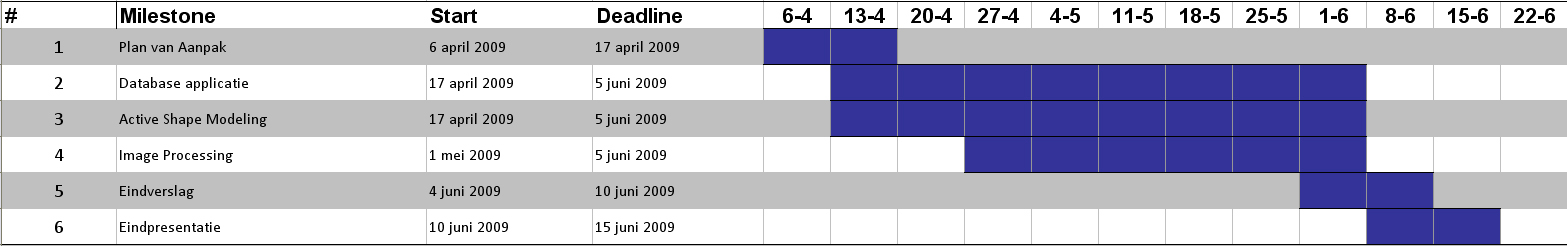
\includegraphics[width=0.9\textwidth]{ganntafter}

\newpage
\section{Aanpak}
\label{Aanpak}
Een van de eerste beslissingen die moest worden genomen is de architectuur van het systeem. Al snel bleek dat de opdrachtgever een voorkeur had voor een webapplicatie die door het hele Erasmus MC op het netwerk simpel en snel gebruikt kon worden. 
Voor onze Image Processing kregen wij het advies van Dr. Botha om een aantal Python bibliotheken te bekijken en deze indien mogelijk te gebruiken. 

De combinatie van deze feiten leidde ons richting Django, dit is een python framework voor het bouwen van websites in Python. Na wat research en de ervaringen die \'{e}\'{e}n van de projectleden al had met Django hebben we ervoor gekozen om Django te gaan gebruiken. 

Voor wat betreft de visuele interactie hebben we gekeken naar verschillende Javascript bibliotheken, mede door de uitgebreide ervaringen van diverse leden hebben we uiteindelijk gekozen voor de combinatie van Prototype en Scriptaculous.

Tijdens het project bleek uiteindelijk dat er behoefte was aan een tekenapplicatie binnen de omgeving en deze was niet te realiseren via Javascript en is er uiteindelijk ook nog een Flash applicatie geschreven welke communiceert met Javascript.

\subsection{Project gerelateerd}
In de begin periode hebben wij ons ingelezen op de basis anatomische kennis die nodig was om de experts van het Erasmus MC te kunnen volgen. Hierbij hebben we vooral veel gebruik gemaakt van de kennis van \'{e}\'{e}n van de groepsleden, die voor ze aan deze studie begon drie jaar. Ook zijn we een dag langs geweest bij het EMC en hebben daar een rondleiding gehad door het laboratorium en de snijzalen waar onderzoek wordt gedaan. 

Een andere uitdaging was de relatief grote groep studenten voor dit project. Om te voorkomen dat we elkaar te veel in de weg zouden zitten hebben we de diverse delen van het project opgesplitst en de taken duidelijk verdeeld. Daarnaast hebben we gebruik gemaakt van software zoals Trac, dit is een Project Management Systeem. Daarnaast was een locatie geregeld op de TU Delft waar we iedere dag hebben gewerkt en waar we elke ochtend een werkoverleg konden hebben voor wat er die dag zou gebeuren. Hierdoor bleef iedereen goed op de hoogte van de status van het gehele project.

\subsection{Database systeem}
Het database systeem is het onderdeel van het project dat dient om de gebruikte foto's overzichtelijk in te delen in verschillende projecten. Hiervandaan wordt de gebruiker in staat gesteld om de handelingen te verrichten die nodig zijn om analyse te plegen op  foto's. Typische handelingen zijn bijvoorbeeld: 

\begin{itemize}
\item Aangeven van herkenningspunten bij de foto's
\item Afbeeldingen tekenen over foto's om belangrijke gebieden aan te geven
\item Verschillende doorzichtige foto's over elkaar heenleggen om de verschillen te bekijken
\end{itemize}

Zoals in de paragraaf Aanpak al aangegeven zouden we gaan werken met Django en moest het product beschikbaar worden als webapplicatie. Django is een MVC LEG UIT!!! opgebouwde taal met een duidelijk abstractie laag voor het database gedeelte. Na diverse brainstorm sessies zijn we uiteindelijk uitgekomen op een klasse diagram wat de basis zou gaan vormen voor het database systeem. Het diagram staat in bijlage B.
Voor de interface hebben we ervoor gekozen om veel gebruik te maken van Javascript en zijn bibliotheken. Dit gaf ons eenvoudige toegang tot diverse visuele effecten, zoals drag en drop, fade en de sliders). Daarnaast konden we met behulp van Javascript gebruik maken van de AJAX techniek, hiermee konden server requests sturen en de pagina updaten zonder dat de gebruiker hier last van had.

\subsection{Image Processing}
De doelen op Image Processing gebied waren het in kaart brengen van de variaties per landmark en het morphen van getekende structuren (bijvoorbeeld zenuwen of venen) naar een standaardview waarop bijvoorbeeld structuren die van verschillende benen afkomen toch op \'{e}\'{e}n been kunnen worden afgebeeld.

\subsubsection{Point Distribution Model}
Om het eerste doel te bereiken hebben we gebruik gemaakt van een sub-onderdeel van een volledig Active Shape Model, namelijk het Point Distribution Model. Het Active Shape Model is ontwikkeld door Tim Cootes, in de paper An Introduction to Active Shape Models licht hij de theorie toe.\cite{introASM}

Waar het Active Shape Model zich bezighoud met het automatisch herkennen van structuren uit een foto, is het Point Distribution Model\cite{pdm} in staat gegeven een aantal landmarks (van hetzelfde type) op verschillende foto's het gemiddelde en de hoofdassen van variatie weer te geven. Een landmark is hierbij een punt dat zo is gekozen dat het in iedere foto te vinden is en duidelijk op ieder fotovoorbeeld te vinden is. De landmarks die nodig zijn voor het Point Distribution Model moeten hierbij informatie geven over het verloop van een structuur, bijvoorbeeld het aangeven van het verloop van een bepaalde vene.

\subsubsection{Thin Plate Spline Transformatie}
Om het tweede doel te bereiken, het morphen van getekende structuren is er gebruik gemaakt van een Thin Plate Spline transformatie. Om de Thin Plate Spline transformatie uit te voeren zijn landmarks nodig die bepalend zijn voor de vorm van een object. Hierbij kan gedacht worden aan een set van landmarks die bestaat uit bony landmarks (landmarks die voortkomen uit de anatomie van het menselijk lichaam en voelbaar zijn vanaf de buitenkant), landmarks die de grenzen van het object aangeven en landmarks die zich op gelijke afstanden tussen voorgaande landmarks bevinden. 


\subsection{Tekenen}
Impliciet zit er in dit doel nog een Image Processing doel verwerkt, namelijk het aangeven van lijnen, gebieden of punten die interessant zijn voor de onderzoeker. We hebben ervoor gekozen om de onderzoeker dit in de browser te laten doen als ge�ntegreed tekenprogramma. Hierbij zal het mogelijk zijn elke foto als achtergrond te kiezen en hieroverheen met ��n kleur bepaalde gebieden aan te geven.

Binnen browsers zou dit tekenprogramma gemaakt kunnen worden door gebruik te maken van Canvas, een onderdeel dat tot een nieuwe HTML-standaard behoort, maar nog niet ondersteund wordt door Internet Explorer 6. Omdat we tijdens de keuze van de techniek er vanuit gingen dat het systeem in IE 6 moest draaien hebben we gekozen om niet Canvas maar Flash te gebruiken. Dit vereis een plugin in de browser, maar bijna iedereen heeft deze plugin.

Over de theoretische achtergrond van de verschillende gebruikte technieken is meer te vinden in het ori\"{e}ntatieverslag. De implementatie komt aan bod in de volgende sectie.





\newpage
\section{Implementatie}
\label{Implementatie}
In de tweede week van het project zijn we echt begonnen met het bouwen van het systeem. 
We zijn begonnen met zogenaamde spike solutions (snelle simpele oplossingen om een deelprobleem op te lossen) van verschillende basis functionaliteiten, zoals het uploaden van afbeeldingen en het plaatsen van landmarks op geplaatste afbeeldingen met behulp van drag \& drop. 
In een later stadium hebben we voor de grotere uitdagingen spike solutions geschreven.
Hieronder vallen onder andere het morphen van foto's en het visualiseren van het Point Distribution Model. 
Als een spike solutions werkte, werd deze aan het bestaande systeem gekoppeld.
Op deze manier hadden we in een vrij korte tijd een basis systeem met basis functionaliteiten. 
Zo konden we ons vervolgens concentreren op de Javascript functies die zouden gaan zorgen voor de AJaX afhandeling en de visuele effecten.

\subsection{Project gerelateerd}
\label{implementatie_project_gerelateerd}
Daar waar het mogelijk en handig was, hebben we geprogrammeerd in tweetallen. 
Tijdens de implementatie fase hebben we veel gebruik gemaakt van de beschikbare whiteboards.
Deze waren handig voor het brainstormen en als iemand vastliep, kon het probleem getekend en uitgelegd worden. 
Dit alles zorgde voor een goede synergie en hierdoor hield iedereen de motivatie die hij had goed vast.
Tijdens de implementatie fase hebben we veel contact gehad met de leden van het \casamproject en zijn er verschillende tussentijdse presentaties geweest. 
Steeds hebben we na zo'n presentatie een uitgebreid overleg gehad over de stand van zaken en ge\"{e}valueerd  hoe het project er voor stond. In sommige gevallen hebben we ook onze prioriteitenlijst aangepast aan de hand van deze vergaderingen.

\subsection{Database systeem}
\label{implementatie_database_systeem}
Voordat we konden beginnen met het database systeem, hebben we eerst een database model gemaakt. De eerste versie van dit model is te zien in Figuur \ref{brainstorm_klassediagram}.
De uiteindelijke versie van dit model is te zien in Figuur \ref{databasediagram}.
Een aantal van de belangrijkste wijzgingen zijn:
\begin{description}
  \item[Measurement types] In het originele model was er een algemeen MeasurementType bedacht, waar alle 3 de types van overerven. 
  In het uiteindelijke model was er nog wel ruimte voor MeasurementTypes, maar zijn dit types geworden die aangemaakt kunnen worden door de gebruiker.
  De MeasurementTypes zoals die bedacht waren bestaan uiteindelijk alleen nog uit Measurements en Bitmaps, waarvan Bitmaps overerft vanuit Image, in plaats van een algemeen MeasurementType.
  \item[Measurements] De Measurements zelf zijn nu wat in het originele model een PointMeasurement heette.
  Ook de ProjectMeasurementsList is uit het model verdwenen, en vervangen door de algemene PotentialMeasurements.
  \item[Images] Het algemene type Image is in het uiteindelijke model gespaard gebleven.
  De Pati\"{e}nt die echter aan een OriginalImage hing, is gesneuveld, omdat dit niets toevoegde aan het systeem.
  Ook hebben we besloten om EditedImages niet op te slaan, en in plaats daarvan States te bewaren.
  \item[States en Projectfiles] States zijn samen met de Projectfiles aan het model toegevoegd.
  Hierbij zijn de States bedoeld om de huidige configuratie van zichtbare foto's, Bitmaps en Measurements op te slaan en weer op te halen.
  De Projectfiles zijn bedoeld voor de export van een project.
  \item[Users] In het originele model zou het user-management door Django geregeld worden.
  Tijdens de implementatie is gebleken, dat we toch nog een UserProfile moeten toevoegen.
  In dit UserProfile wordt opgeslagen welke Gebruiker welke rechten heeft op welk project.
\end{description}
Andere aspecten van het database systeem worden hieronder toegelicht.

\subsubsection{Verschillende doorzichtige foto's over elkaar heen leggen om de verschillen te bekijken}
Voor de weergave van afbeeldingen binnen het project is er bedacht dat er meerdere afbeeldingen tegelijk zichtbaar moesten kunnen zijn.
Hiervoor is er vastgesteld dat er verschillende afbeeldingen over elkaar heen gelegd gaan worden, met een door de gebruiker in te stellen volgorde en doorzichtigheid.
Om dit te kunnen realiseren hebben we eerst voor elke afbeelding in het project een eigen slider gemaakt, die pas geladen wordt op het moment dat de afbeelding zichtbaar wordt gemaakt. 
Met deze slider kan de gebruiker vervolgens zelf instellen met welke doorzichtigheid de corresponderende afbeelding zichtbaar gemaakt moet worden.
Deze slider was een onderdeel van de Scriptaculous bibliotheek, waar in het project vaker gebruik van gemaakt is.
Hierna moest het mogelijk gemaakt worden om de volgorde van de weergegeven afbeeldingen aan te passen.
Dit hebben we gedaan door van de lijst met afbeeldingen in het linker frame een Sortable te maken.
Dit heeft als voordeel dat de volgorde nu bepaald kan worden door de gewenste zichtbare afbeelding naar boven te slepen.
Ook wordt de volgorde van de lijst automatisch aangepast op het moment dat er een afbeelding zichtbaar wordt gemaakt, door deze afbeelding naar boven te verplaatsen in de lijst.
De bovenste afbeelding van de lijst wordt altijd ook de bovenste afbeelding van alle zichtbare afbeeldingen, zodat de bovenste afbeelding altijd de actieve afbeelding is, waarop de bewerkingen worden gedaan.

\subsubsection{Herkenningspunten bij de afbeeldingen}
Voor het toevoegen van herkenningspunten aan de afbeeldingen hebben we ervoor gekozen om deze op te slaan in een apart model in de database.
Aan dit model zit een koppeling met de MogelijkeMetingen vast, evenals met de afbeelding waar het punt bij hoort en het project.
Om een herkenningspunt (landmark) op te kunnen slaan, moeten deze eerst bestaan.
Als er een foto geladen is in het scherm, wordt hier met JavaScript een listener aan gekoppeld die reageert als er op de foto geklikt wordt.
Deze listener wordt weer van de foto afgehaald op het moment dat er een andere foto overheen geladen wordt, en er een andere foto bestempeld wordt als actieve laag.
Aan deze foto wordt dan weer een listener gekoppeld, die de muisklik op de foto afvangt.
Als er op de geladen foto's wordt geklikt, wordt de listener (van de foto van de actieve laag) geactiveerd en wordt er een popup-schermpje getoond waarin de benodigde informatie voor het landmark staat.
In deze popup dient er een MogelijkeMeting gekozen te worden van het landmark, en wordt er onzichtbaar een ID meegegeven van de foto.
Als er in de popup dan op 'Save' geklikt wordt, wordt er eerst in de JavaScript code gekeken of het landmark al bestaat of niet.
Voor een landmark dat al bestaat, wordt er een 'repositioning'-change aangemaakt, waarin de nieuwe co\"{o}rdinaten worden opgeslagen, terwijl er voor een nieuw landmark een 'positioning'-change wordt aangemaakt.
Hierna wordt er een AJaX call naar de server gedaan.
Op de server wordt er vervolgens gekeken of er al een landmark bestaat, met het gegeven foto-ID en de gegeven MogelijkeMeting.
Is dit zo, dan wordt dit landmark opgehaald, en aangepast.
Bestaat er nog geen landmark met de gegeven parameters, dan wordt er een nieuwe aangemaakt.
In beide gevallen wordt het bewuste landmark vanuit de database terug gegeven naar JavaScript, door middel van een JSON-string.
Als het landmark opgeslagen kon worden op de server, wordt de hiervoor aangemaakte change in JavaScript ook opgeslagen.
Vervolgens wordt voor een bestaand landmark de positie aangepast.
Voor een bestaand landmark wordt er een nieuw measurement aangemaakt, dat op de goede plaats onder de afbeelding wordt geplaatst.

\subsubsection{Afbeeldingen tekenen over foto's om belangrijke gebieden aan te geven, ook wel bitmaps genoemd}

Een plek in ons systeem waar de samenwerking van verschillende deelsystemen en zelfs verschillende talen goed zichtbaar wordt is de manier waarop de Flash-applicatie gebruikt wordt om bitmaps te tekenen. Hieronder staat dit in een sequence-diagram weergegeven.

Het eerste deel van het diagram toont op welke wijze het bestaan van bitmaps geladen wordt in de JavaScript-omgeving. De rest van het diagram toont wat het systeem doet als de gebruiker het tekenen of bewerken van een bitmap kiest.

Eerst wordt in de HTML-pagina een object ingevoegd waarin de Flash-applicatie geladen wordt. Vervolgens laadt de Flash-applicatie de afbeelding waar op getekend gaat worden. Als de gebruiker vervolgens kiest om de bitmap op te slaan wordt de tekening naar de server verzonden, en als deze succesvol opgeslagen is krijgt de Flash-applicatie een bevestiging waarop deze een melding naar de JavaScript-omgeving gemaakt wordt met het verzoek de Flash-applicatie te sluiten. Dit is de laatste actie die in het diagram beschreven wordt.

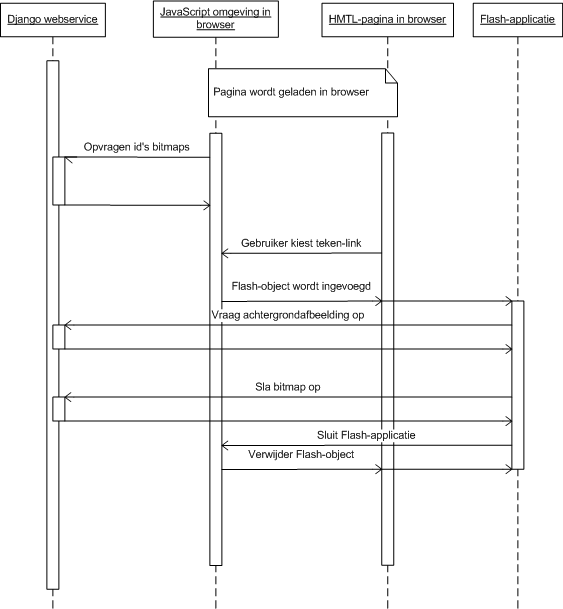
\includegraphics[width=100]{ sequencediagram }


\subsubsection{Toevoegen van relevante papers en websites}
Voor het toevoegen van papers en websites aan een project hebben wij gekozen om deze ook in een apart model in de database op te slaan.
In dit model zit een verwijzing naar het project waar de toevoeging bij hoort en een verwijzing naar de toevoeging zelf.
Deze verwijzing bestaat in het geval van een website uit een URL, en in het geval van een paper uit een link naar de paper die op de lokale server wordt opgeslagen.
\subsubsection{Tags toevoegen aan projecten om ze te categoriseren}
Om een grote verzameling projecten overzichtelijk te houden was het noodzakelijk om een aantal trefwoorden (tags) aan een project te koppelen.
Ook moest het mogelijk zijn om onderlinge verbanden tussen projecten te leggen door middel van dezelfde tags.
Op deze manier kan er makkelijk gezocht worden op de tags en worden alleen de overeenkomstige projecten getoond.
Bij het aanmaken van een project kan er gekozen worden uit de selectie van bestaande tags, zodat een project direct makkelijk gevonden kan worden.
Voor het aanmaken van nieuwe tags is het wel nodig om het project te openen.
Deze nieuwe tags kunnen daarna direct aan andere projecten worden gekoppeld.
\subsubsection{States}
Een onderdeel dat erg lastig bleek te implementeren waren de states.
States zijn de manier om, wanneer een interessante samenstelling van foto's, landmarks, bitmaps etc. op het scherm staat, deze op te slaan om het later terug te kunnen halen.
Omdat de software voornamelijk was ontworpen om handelingen te verrichten bij interactie van de gebruiker, bleek het erg moeilijk te zijn om via code een eerder opgeslagen state te herstellen.
Om dit mogelijk te maken is een ander HTML en JavaScript model nodig, waarvoor een aanbeveling wordt gedaan in hoofdstuk 7.
Omdat deze aanpassingen nog niet doorgevoerd zijn is een tijdelijke oplossing ge\"{i}mplementeerd die een deel van de HTML structuur opslaat wanneer de gebruiker erom vraagt, en deze kan later in een popup weer worden getoond zodat een soort van statische state ontstaat waar niet in verder gewerkt kan worden.
Een andere manier zou zijn om de state op te slaan in een plaatje, waarbij het renderen van de browser wordt nagebootst door de Python Image Library.
Omdat deze manier een moeilijkere implementatie heeft dan het kopie\"eren van de HTML, en niet per s\'e een beter resultaat oplevert, is ervoor gekozen om dit niet te implementeren.
\subsubsection{Afstanden meten in foto's}
We hebben een spike solutions geschreven voor het meten van afstanden in foto's. 
Mede door tijdsgebrek en de afhankelijkheid van andere spike solutions zijn we er niet aan toegekomen om dit te implementeren. 
In sectie \ref{customjaap} gaan we hier verder op in.

\subsection{Image Processing}
\label{implementatie_image_processing}
Image Processing was \'{e}\'{e}n van de grootste uitdagingen van het project. Niemand had ervaring met de verschillende bibliotheken of uitgebreide ervaring met dit aspect van Image Processing. Er waren verschillende opties om de benodigde technieken te implementeren. Zo konden we ze zelf implementeren met behulp van Numpy\cite{numpy} of gebruik maken van grotere bibliotheken zoals Insight Segmentation and Registration Toolkit (ITK)\cite{ITK} of de Visualization Toolkit (VTK)\cite{vtk}. Verder was er nog de Python Imaging Library (PIL)\cite{pil} die geschikt is om eenvoudige beeldbewerking te doen. Uiteindelijk is er, mede op advies van Dr. Botha, gekozen voor PIL in combinatie met de VTK bibliotheek. Om aan de vraagstelling te kunnen voldoen, het in kaart brengen van de variaties per landmark en het kunnen projecteren van getekende gebieden op \'{e}\'{e}n gemiddeld plaatje, hebben we gekozen om een deel van de methode Active Shape Modeling, genaamd Point Distribution Models, toe te passen in combinatie met Thin Plate Spline transformaties. Hierdoor is het mogelijk voor de onderzoeker om op een wiskundig verantwoorde manier anatomische structuren op een gemiddelde te projecteren en de variaties per landmark te visualiseren.
Al snel bleek dat er veel onderzoek nodig was om de theorie achter Principal Component Analysis, Active Shape Models, Point Distribution Models en de Thin Plate Spline Transformaties te doorgronden. Ook kostte het enige extra tijd om met de VTK bibliotheek bekend te raken.

\subsubsection{Point Distribution Model}
Om het Point Distribution Model te maken is een set nodig van verschillende landmarks waarvan de variaties en de gemiddelden interessant zijn om weer te geven. Het is van belang om de landmarks zo te kiezen dat ze makkelijk zijn te vinden in elke foto en belangrijke punten aangeven op de structuur waar het om gaat. De gebruiker kan landmarks in de foto aangeven door eerst een landmarktype aan te maken, dan een landmark van een bepaald type en hierbij aan te geven of het een shapedefining landmark is of niet. Nadat de gebruiker in de foto's de gewenste landmarks heeft aangegeven kan hij door 'Analyse selected landmarks' aan te klikken het Point Distribution Model van de geselecteerde landmarks laten uitrekenen en weergeven.

Op dit moment wordt in JavaScript gecontroleerd welke images en landmarks geselecteerd zijn en wordt er via een AJaX request de id's van de afbeeldingen en de geselecteerde landmarks per afbeelding doorgegeven. Aan de hand van de id's van de afbeelding en de landmarks worden vervolgens de bijbehorende objecten uit de database gehaald. In de view wordt getest of de geselecteerde landmarks wel geschikt zijn om een Point Distribution Model van te maken. Dit is bijvoorbeeld niet zo als: er geen landmarks geselecteerd zijn, er te weinig landmarks geselecteerd zijn van een type of de geselecteerde landmarks van een geheel ander type zijn. In elk van deze gevallen wordt er een foutmelding aan de gebruiker gegeven in de vorm van een JavaScript alert met de aard van de fout, zodat de gebruiker zijn selectie kan aanpassen.

Als de juiste landmarks zijn geselecteerd wordt er allereerst via de co\"{o}rdinaten van de landmarks per afbeelding een vtkUnstructuredGrid aangemaakt met de desbetreffende punten erin als vertices. Vervolgens wordt over deze grids de Generalized Procrustes Analysis uitgevoerd via het vtkProcrustesAlignmentFilter. Dit zorgt ervoor dat de gevonden modi van variatie onafhankelijk van de positie en de rotatie van de objecten zijn. Door ervoor te kiezen om de mode op RigidBody te zetten blijft echter wel de grootte van de structuren behouden. De opgeslagen grids zijn nu iteratief getransleerd en geroteerd naar elkaar toe.

Nu is het tijd om de Principal Component Analysis (PCA) op de aligned grids uit te voeren, dit is gedaan met behulp van het vtkPCAAnalysisFilter. Uit het resultaat kunnen de gemiddelde posities per landmark gehaald worden. We hebben er voor gekozen om de eerste twee modi van variatie te berekenen, de hoofdmodus van variatie (eerste mode) zorgt altijd voor de grootste verandering en is de eigenvector met de grootste eigenwaarde die uit de PCA komt. Om deze variaties te berekenen vragen we de GetParameterisedShape en berekenen we hiermee voor de eerste en tweede modus de extremen, dit zijn plus en min 3 standaarddeviaties van het gemiddelde.

Nu we de benodigde co\"{o}rdinaten hebben (gemiddelden en extremen) kunnen we beginnen aan de visualisatie van de landmarks. Dit wordt gedaan met behulp van de PIL. Aan de hand van de afmetingen van de originele foto's en de gegeven co\"{o}rdinaten wordt voor het gemiddelde een ellips getekend. Tussen de extremen van de twee hoofdmodi van variatie wordt een lijn getekend. De lengte van deze lijn geeft de grootte van de mogelijke variatie aan op basis van de voorbeelden uit de gegeven landmarks. Door de ellipsoids en lijnen weer te geven met een doorzichtige achtergrond is het vervolgens mogelijk om deze als een overlay over de images te projecteren. De overlay wordt opgeslagen in de database en is beschikbaar voor weergave vanuit de interface.


\subsubsection{Thin Plate Spline Transformatie}
Om de daadwerkelijke morph uit te voeren van de getekende structuren moesten we eerst een transformatie uitvoeren om verschillen in translaties en rotaties tussen de verschillende foto's te verwijderen. Na overleg met dr. Botha is besloten om dit niet via Generalized Procrustes Aligment te doen, maar om \'{e}\'{e}n foto (in dit geval de eerste) als voorbeeld te nemen en alle andere getekende structuren naar deze foto te morphen.  Hierdoor ontstaat een foto met een bestaande anatomie. Dit heeft een groot voordeel ten op zichte van het morphen van alle foto's naar een gemiddelde, want dan onstaat er een gemiddelde foto zonder bestaande anatomie. Helaas kwam de implementatie van dit onderdeel van het project te laat om ook nog het Point Distribution Model volgens deze gedachte te implementeren. 

In grote lijnen werkt de implementatie op dezelfde manier als die van het Point Distribution Model met een paar verschillen. Wederom worden landmarks uit de interface ingelezen en opgehaald. Er wordt naast de eerdergenoemde checks ook nog gekeken of de landmarks wel allemaal shapedefining zijn. Voor het morphproces worden namelijk een ander soort landmarks gebruikt dan voor het berekenen van het Point Distribution Model. De shapedefining landmarks zijn landmarks die kenmerkend zijn voor de vorm van het hele object (je kunt bijvoorbeeld denken aan de bony landmarks van het been met daartussen op gelijke afstanden geplaatste landmarks op de omtrek van het been). 

Met de gevonden foto's en de bijbehorende landmarks worden de co\"{o}rdinaten van de landmarks ditmaal direct in vtkPoints objecten gezet. Deze vtkPoints worden gebruikt in de vtkLandmarkTransform. Als source landmarks worden per foto de vtkPoints gebruikt en als target de vtkPoints van het gekozen active image. Via vtkImageReslice wordt de daadwerkelijke transformatie uitgevoerd. We kiezen Nearest Neighbour als interpolationmode om ervoor te zorgen dat de kwaliteit van de getekende structuren niet verslechtert. Net als bij het Point Distribution Model wordt de mode op RigidBody gezet om informatie over de grootte niet te verliezen. Vervolgens wordt de output van deze transformatie gebruikt als source voor de daadwerkelijke morph. Het morphen zelf wordt ge\"{i}mplementeerd met behulp van de vtkThinPlateSplineTransform. De source landmarks zijn gelijk aan de output van de eerste transformatie, voor de target landmarks zijn weer de landmarks van het gekozen active image gekozen. Via de vtkImageReslice wordt nu het eindresultaat bereikt, de bitmaps van alle geselecteerde foto's worden nu, gemorpht naar de active image, weergegeven.


\subsubsection{Tekenen}
Vanuit de applicatie kan op twee manieren de Flash-applicatie gestart worden. Het kan door in het rechter scherm met Possible Measurements een nieuwe bitmap aan te maken terwijl een afbeelding actief is. De tweede methode is om een bestaande bitmap die aan een image gekoppeld is te bewerken door in het linker vak op de edit-knop te klikken.

Dit opent de Flash-applicatie waaraan in een HTML-tag argumenten meegegeven worden, zoals een verwijzing naar de achtergrondfoto en optioneel een bestaande bitmap. In de Flash-applicatie kan vervolgens in een aparte laag getekend worden in \'{e}\'{e}n kleur. Als op de Save-knop gedrukt wordt scant de Flash-applicatie de hele tekenlaag per pixel om een compacte representatie te maken van de tekening. Deze wordt vervolgens naar de server gestuurd met een HTTP-POST, samen met andere gegevens. Als de server dit succesvol afvangt en verwerkt krijgt de Flash-applicatie een antwoord en roept de applicatie een JavaScript-functie in de browser aan die de Flash-applicatie afsluit.

Een probleem dat optrad bij grote foto's was dat het afscannen van de tekenlaag enkele seconden kon duren. Om deze reden is er een extra optimalisatie ingebouwd: de applicatie houdt bij in welk gebied getekend is door een minimale en maximale x en y bij te houden. Op deze manier hoeft maar een beperkt deel van de laag gescand te worden, wat meestal significant veel tijd bespaard. In het ergste geval is over de hele foto getekend en dan levert deze optimalisatie geen winst maar ook geen verlies op. Omdat de applicatie bij elke muisbeweging wel de minimale en maximale co\"{o}rdinaten bijwerkt kan het zijn dat zij iets minder gevoelig is voor de tekenbeweging zelf, maar uit tests bleek dat dit niet storend was.

Als een al bestaande bitmap wordt geladen worden daarbij ook de vorige minimale en maximale co�rdinaten geladen. Binnen dat bereik scant de Flash-applicatie de oude bitmap pixel voor pixel af totdat de eerste gekleurde pixel gevonden wordt om de vorige kleur te pakken te krijgen. 

\subsubsection{Tekenen: de serverkant}
De POST van de Flash-applicatie is zo compact mogelijk opgebouwd. Deze bestaat uit een header met de afmetingen en de co\"{o}rdinaten van het tekengebied. De data zelf bestaan uit nummers die aangeven hoeveel pixels aaneengesloten gekleurd zijn of niet. Op deze manier bestaat dus een compleet gekleurde bitmap maar uit \'{e}\'{e}n getal.

De server bouwt deze representatie om naar een grote string met \'{e}\'{e}n karakter per pixel, die met een methode uit de PIL opgeslagen kan worden als GIF-afbeelding. Er wordt ook een palet gekoppeld aan de GIF-afbeeldingen met als 255'ste waarde de kleur die in de Flash-applicatie gekozen is. Op deze manier wordt de bitmap die in de Flash-applicatie nog uit meerdere kleuren kon bestaan opgeslagen als een GIF-afbeelding met de laatst gebruikte kleur.

\newpage
\section{Aanbevelingen} %7
\label{Aanbevelingen}
Hieronder een korte toelichting op werkzaamheden waar wij niet aan toe zijn gekomen. 
Sommige van deze werkzaamheden zijn niet gebeurd omdat ze buiten het bereik van het project vielen of omdat ze tijdens het project bedacht werden. 
In enkele gevallen hadden we wel gepland om het werk te doen maar zijn we er niet aan toe gekomen.  

In de toelichting geven we een korte samenvatting van wat er in brainstorm sessies en/of vergaderingen over is afgesproken. 
Wij hopen op deze manier dat toekomstige groepen op een eenvoudige en snelle manier kunnen verder werken aan het product.

\subsection{Bestandstypen van foto's} %7.1
Op dit moment kan de morph-functie alleen foto's aan van het JPEG-formaat. 
Alhoewel dit het meest gebruikte formaat is zou het een verbetering zijn als het systeem ook met andere formaten om kan gaan. 
Een probleem is, dat de foto's bij het uploaden wel de extensie 'jpg' krijgen, maar het geen jpeg foto's zijn. 
Het kan nu gebeuren dat er een gif-afbeelding wordt geupload, die vervolgens de extensie jpg krijgt. 
Hierdoor geeft de vtkJPEGReader een error, en kan er met dit plaatje niet gemorphd worden. 
Het weergeven van de afbeelding in de browser gaat wel goed, waardoor het voor de gebruiker niet duidelijk is dat er eigenlijk iets mis is met de afbeelding.

Een oplossing zou kunnen zijn om bij het uploaden van de afbeelding de Python Imaging Library te laten kijken naar de foto, en deze om te laten zetten naar een echt jpeg bestand. 
Het gevaar hierbij is, dat er door de compressie van het JPEG-formaat er aan scherpte van de foto verloren gaat.
Een oplossing voor dit probleem zou kunnen zijn om helemaal geen jpeg-bestanden meer op te slaan, en alle foto's te laten omzetten naar het PNG-formaat. Bij deze omzetting gaat vrijwel geen informatie in de foto verloren, en voor dit formaat zijn dezelfde VTK-library's beschikbaar als voor het jpeg formaat.

Dit is echter een probleem waar wij binnen het project te laat tegenaan liepen, waardoor er geen tijd meer was om dit op te lossen.

\subsection{Verschillende kleuren in flash applicatie} %7.2 <---
Binnen onze applicatie is het op dit moment al mogelijk om een bitmap te tekenen in een willekeurige kleur. 
Wat echter nog niet mogelijk is, is om in \'{e}\'{e}n bitmap meerdere kleuren te gebruiken.
Voor de gebruikers zou het intu\'{i}tiever zijn om dit wel te kunnen, vooral omdat er bij het tekenen van de bitmap wel met verschillende kleuren gewerkt kan worden.
Het moet de gebruiker dan expliciet verteld worden dat de hele bitmap wordt opgeslagen in de kleur waarmee het laatst is gewerkt.
%TODO voor Bastiaan

\subsection{Opslaan van een lege bitmap}
Op dit moment is het niet mogelijk om een bestaande bitmap te bewerken naar een lege, omdat dan in de submit de minimale en maximale co�rdinaten gezet zijn naar defaultwaarden die de server niet aankan. Daarom wordt nu afgevangen dat er een lege bitmap is gesubmit, maar deze wordt verder niet opgeslagen.

De enige reden om een lege bitmap op te slaan is om deze te verwijderen, maar zoals elders beschreven moet dat nu nog via de admin-interface gedaan worden. Lege bitmaps opslaan is niet de manier, en wegens de huidige implementatie wordt de lege dump dus ook niet opgeslagen.

Het systeem zou verbeterd kunnen worden door de Save-knop weg te halen uit de Flash-appliactie als er niets is getekend. Dat maakt het voor de gebruiker duidelijker dat opslaan van een leeg plaatje niet kan. Er moet sowieso ook nog een verwijderknop in het systeem gemaakt worden. Als deze duidelijker aanwezig is voorkomt dit dat de gebruiker een lege bitmap op zou willen slaan.

\subsection{Te grote foto's inladen in de flash-applicate}
Een vervelende beperking van de Flash-applicatie waar we op een erg laat moment achter kwamen is dat de maximale grootte van een afbeelding die je in Flash kan laden 2880 x 2880 pixels is. De afbeeldingen die gebruikt zullen worden in het systeem zijn doorgaans groter, wat erin resluiteert dat alle pixels die buiten de marge het ondersteunde gebied vallen gewoon niet geladen worden. Het wordt dan niet mogelijk om buiten dit gebied te tekenen en de naar de server geposte dump is ook maximaal 2880 x 2880 pixels.

Er zijn grofweg twee oplossingen te bedenken. De makkelijkste is het resizen van de image naar maximaal 2880 x 2880 pixels voordat deze door de Flash-applicatie geladen wordt. Dit kan het systeem al. Het probleem komt aan de serverkant wanneer de server de geposte dump terug moet rekenen naar volledige grootte. Deze moet opgevraagd worden bij de orignele afbeeldingen die in verkleinde vorm als achtergrond diende. Het probleem bij deze aanpak is dat er geen pixelprecisie meer is in het tekenen over de afbeeldingen, omdat deze geresized wordt. Omdat de resolutie van de afbeeldingen redelijk groot is, is dit geen groot probleem.

%titels zijn voorstellen, kunnen gewijzigd worden
\subsection{statistische data bij landmarks} %7.5
Een bekende wens vanuit de gebruikers bij het EMC is dat er statistische data opgeslagen kan worden bij de aangegeven landmarks.
Deze data heeft betrekking op de diepte waarop een vene op verschillende punten in het been ligt.
In de huidige situatie wordt deze data apart in een Excel-sheet bijgehouden en naar een statisticus gebracht.
Deze maakt hier vervolgens in aparte software (SPSS)\ref{spss} een aantal grafieken van, die de gebruiker bij de andere data op zou willen slaan.
In de toekomst zou het mogelijk moeten zijn om deze data bij de landmarks zelf op te slaan.
In een ideale situatie zouden zelfs de grafieken in het systeem moeten verschijnen, waarna de gebruikers van een willekeurig punt op de grafiek de waarde op kunnen vragen.

Vanwege de complexiteit van het opslaan van de statistische data, het later genereren van de bijbehorende grafieken en het kunnen opvragen van de waardes op een willekeurig punt, hebben wij hier nog geen stappen voor ondernomen.
Een volgende groep zou kunnen beginnen met het enkel toevoegen van de data en deze overzichtelijk weer te geven, zonder hier grafieken van de maken.
De analyse van deze data en het hieruit produceren van bruikbare data, is daarna weer een probleem apart.
Wat zelfs voor een eerste opzet waarschijnlijk een heleboel onderzoek nodig heeft.
Het enige licht wat wij nu al een beetje op de zaak kunnen laten schijnen is dat er een PyCha module bestaat waarmee in Python grafieken gemaakt kunnen worden.

\subsection{uitwerken afstand meet applicatie} %7.6
Vanuit het EMC was de wens gekomen om het mogelijk te maken om in foto's afstanden te meten.
Dit zou dan gebruikt kunnen worden bij de statistische data, zoals dit hierboven al beschreven is.
Aangezien dit een van de eerste vragen van het EMC was hebben we hier al even naar gekeken en er een spike solution voor gebouwd.
Hier zat echter nog een niet acceptabele meetfout in, waardoor de functie niet in de uiteindelijke interface terecht is gekomen.

Er waren echter wel een aantal manieren waarop de nu aanwezige meetfout waarschijnlijk teruggedrongen kon worden:
\begin{description}
	\item[verplaatsen lineaal] Op de foto's van het EMC is een lineaal zichtbaar. 
	Echter deze lineaal ligt op de verkeerde positie ten op zichte van waar gemeten wordt, er is namelijk een diepte verschil. 
	Ook ligt de lineaal niet recht onder de camera, dit zorgt voor een hoek in de kalibratie stap.
	\item[fout zichtbaar maken] Op dit moment wordt de fout wel uitgerekend. 
	Deze fout zou zichtbaar moeten gemaakt worden aan de gebruiker, zodat hiermee rekening kan worden gehouden.
	\item[opslaan kalibratie] Elke keer als een foto wordt geopend moet de kalibratie stap opnieuw worden uitgevoerd. 
	Hierdoor ontstaat mogelijk onzorgvuldigheid en de kalibratie stap zou moeten worden opgeslagen.
	\item[automatische herkenning] Als de lineaal kan worden herkent door een algoritme dan kan de kalibratie stap geautomatiseerd worden en wordt de menselijke factor verkleind.
\end{description}

\subsection{uitgebreid user management en arts-view mode} %7.7
Wat betreft het huidige user management zijn er nog vele verbeteringen mogelijk.
Momenteel zijn er namelijk 3 gebruikersgroepen aanwezig, die niet altijd evengoed gecontroleerd worden.
Zo is het nu voor een arts ook mogelijk om landmarks toe te voegen aan een project, terwijl dit niet zou moeten mogen.
Ook moet het toekennen van rechten aan projecten beter en duidelijker gaan verlopen.
Daarnaast zou een gebruiker ten alle tijden zijn eigen wachtwoord aan moeten kunnen passen, terwijl dat nu alleen door een 'beheerder' gedaan kan worden.

Zoals al aangegeven is er voor het user management al wel een begin gemaakt, maar dit moet eigenlijk nog uitgebreid worden.
Een deel van deze uitbreiding zou ook in kunnen houden dat er nauwer wordt samengewerkt met de permissions die in Django aan gebruikers toegekend kunnen worden, omdat hier eigenlijk nog niets mee gebeurd.

Zelf zijn wij door tijdsdruk hier niet goed meer aan toegekomen, en is het eigenlijk blijven liggen, ondanks dat een degelijke user management in eerste instantie wel een van de eisen het EMC was.

\subsection{verwijderen measurements zonder admin}
Wat betreft het verwijderen van objecten uit het systeem, is er grote winst te behalen.
Zo wordt voor het verwijderen van de volgende objecten nu nog de Django admin-interface gebruikt:
\begin{itemize}
  \item Bitmaps
  \item Landmarks
  \item PDMs
  \item Projects
  \item Tags
\end{itemize}
Van deze objecten wordt er alleen voor projecten ook de mogelijkheid geboden om deze via de normale interface te verwijderen. 
Terwijl eigenlijk alle objecten via de interface verwijderd moeten worden.

Toen wij hier zelf over aan het nadenken waren, kwamen wij tot de conclusie dat er een aantal oplossingen waren die allemaal eigenlijk niet zo goed zouden werken.
De oplossingen waar wij aan gedacht hebben, staan hier onder beschreven:
\begin{description}
  \item[Inline delete] Een van de mogelijkheden is om in de interface achter elke landmark en elke bitmap een rood kruisje te plaatsen.
  Hier hebben wij vanaf gezien, omdat wij vonden dat de gewone gebruikersinterface dan te vol zou worden.
  Verder staan er nergens in de interface kruisjes en hebben we overal managers voor
  \item[Bij de image manager] Omdat de landmarks en bitmaps onderdeel zijn van de afbeeldingen, zou het bij de image manager erbij kunnen.
  Dit zou dan inhouden dat er eerst op de afbeelding geklikt moet worden, waarna er een lijstje met landmarks en bitmaps verschijnt die verwijderd kunnen worden.
  Nadeel hiervan is dat de image manager niet de plek is om dit soort dingen in te regelen, omdat hij bedoeld is voor de afbeeldingen.
  \item[Delete mode]De meest radicale oplossing is om een delete mode toe te voegen aan de interface.
  Het idee is dat je op een knop kan drukken, waarna er een nieuwe interface geladen wordt.
  In deze nieuwe interface kan je dan eigenlijk alles naar een prullenbak slepen, waarna het verwijderd word op het moment dat je deze delete mode weer verlaat.
  Dit klinkt op zich als een leuk idee, echter het zou heel veel tijd gaan kosten.
  Daar komt nog eens bij dat we niet zeker weten of dit wel een idee was wat aan zou slaan bij de gebruikers, en of dit voor de gebruikers wel intu\"{i}tief is.
  \item[Eigen manager] Een eigen manager voor de landmarks en bitmaps is waarschijnlijk het beste idee, maar door de tijdsdruk zijn we ook hier niet aan toe gekomen.
  Het enige tegen deze oplossing was het feit dat er dan nog een link bij zou komen in de interface.
  Gekscherend werd er gezegd dat er bijna behoefte was aan een manager voor de managers, omdat het er inmiddels al zo veel zijn.
\end{description}

\subsection{morphen naar standaard AnatomicalView}
%TODO: NOESKA

\subsection{zoom op meerdere niveau's}
Een leuke en handige uitbreiding voor de nu aanwezige zoomfunctie in de interface, is om het niveau van de zoom in te kunnen stellen.
In het zoom-scherm wordt het huidige plaatje nu twee keer zo groot weergegeven als dat het in werkelijkheid is, maar idealiter is dit in te stellen naar een willekeurige grootte.
Om dit te bereiken is het wellicht het makkelijkst om te beginnen met het zoomen op een aantal vastgestelde niveau's, zoals 150\%, 200\%, 250\% en 300\%.
Dit kan dan later nog uitgebreid worden naar een door de gebruiker in te stellen niveau, binnen vastgestelde grenzen.

Wij hebben dit nog niet aangepakt, omdat er nog een aantal haken en ogen aan de huidige implementatie zitten, namelijk:
\begin{description}
	\item[inladen vaste niveau's] Het inladen van een afbeelding op een aantal vaste niveau's is wat betreft de load nog wel haalbaar, maar voor een willekeurig niveau is dit onhaalbaar.
	\item[inladen geselecteerd niveau] Een alternatief is om de afbeelding met het gewenste zoomniveau op te halen nadat het niveau is ingesteld door de gebruiker.
	Het nadeel hiervan is dat \'{e}\'{e}n afbeelding dan heel vaak opgehaald moet worden, voordat de gebruiker het gewenste niveau heeft gevonden.
	\item[vergroten in venster] Een volgende oplossing is het laten vergroten van de reeds ingeladen afbeelding.
	Het grote nadeel van deze oplossing is dat een afbeelding momenteel wordt ingeladen met een afmeting die afhankelijk is van de afmeting van zijn container.
Als deze dus klein is, wordt er standaard een foto met heel weinig detail ingeladen.
Op het moment dat deze foto vervolgens uitvergroot wordt, blijft er in de uitvergrootte afbeelding te weinig detail over om bruikbaar te zijn.
	\item[verkleinen in venster] Een oplossing die zou kunnen werken, is om de afbeelding altijd op een maximum percentage in te laden  en deze te verkleinen, afhankelijk van het gewenste niveau.
\end{description}

\subsection{schaalweergave in image}
Omdat een afbeelding nu wordt ingeladen op een formaat dat afhankelijk is van het formaat van zijn container, is er vrijwel altijd sprake van een schaalweergave.
Dit wordt echter nergens in het systeem getoond.
Voor de volledigheid van het systeem zou er  bij een afbeelding dus nog een schaal moeten worden weergegeven.
Omdat het daadwerkelijke ophalen van de afbeelding door Python gebeurd is het wellicht het handigst om deze schaal ook door Python te laten berekenen en terug te laten geven aan de website.

\subsection{export on unix import on windows}
Doordat Windows geen ondersteuning heefd voor reverse seeks is het niet mogelijk om een export die gemaakt is op Unix of Mac OS X te importeren op een Windows server. Vermoedelijk kan dit verholpen worden door de inkomende import eerst naar een tijdelijk bestand weg te schrijven, maar dit is niet zeker. Als ook dat niet werkt dan kan er gekeken worden naar een ander bestandsformaat voor import/export (zoals tar.gz).

\subsection{HTML en JavaScript refactor}
Omdat het systeem in korte tijd is ge\"evolueerd naar een uitgebreid systeem is het aan te bevelen om in de toekomst code te herschrijven. Van het scherm dat per project getoond wordt is het het belangrijkst dat het herschreven wordt, omdat hierin de meeste gebruikershandelingen worden gedaan en het onderdeel is dat het meest uitgebreid zal worden. Het is verstandig om een stricte scheiding te maken tussen geladen objecten vanuit de database en de HTML die hiervoor wordt gegenereerd. Het is aan te bevelen om per projectscherm \'{e}\'{e}n controller-object te maken die voor alle mogelijke transacties de administratie van objecten en HTML moet bijhouden. Hierdoor ontstaat een frontend systeem dat consistent is met de backend, iets dat vooral door de realtime natuur van de gebruikte AJaX-technologie een goede administratie vereist. Om de workflow te verbeteren is het tenslotte belangrijk dat de gebruikersinteractie door het hele systeem zo veel mogelijk \'in de pagina zelf gebeurt, zodat de gebruiker voor zo weinig mogelijk acties hele pagina's moet \(her\)laden. Dit is op veel plaatsen in het systeem al gedaan door te werken met popups die in de pagina verschijnen.
\newpage
\section{Conclusie}
\label{Conclusie}
In de afgelopen tien weken hebben wij een systeem gebouwd, dat gebruikt kan worden door het CASAM-project binnen het EMC, ten behoeve van hun onderzoek naar de anatomie.
In onze ogen voldoet het systeem aan de eisen die de opdrachtgever samen met ons heeft vastgesteld. 
In dit project hadden wij op verschillende terreinen grote uitdagingen.
Van project management tot het verwerken van de Image processing in onze applicatie.
Wij zijn van mening dat de meeste van deze uitdagingen gewonnen zijn en dat zij hebben bijgedragen aan een bijzonder product. 
Zoals bij ieder ICT-project is er ruimte over voor uitbreiding en verbetering van het huidige product.
%Deze vervolg werkzaamheden zouden in dezelfde of andere samenstelling kunnen plaatsvinden.
Een volgende groep die aan het project gaat werken zou zelf moeten kijken in welke richting zij door willen gaan.
De punten die genoemd worden in dit verslag kunnen als een uitgangspositie gelden voor de planning van deze werkzaamheden.

\section{Dankwoord}
\label{Dankwoord}
Wij danken: de heer Dr. C.P. Botha, Assistant Professor of Medical TU Delft voor zijn hulp met de visualisatie bibliotheken, de heren Dr. G.J. Kleinrensink universitair docent anatomie aan de Erasmus Universiteit en Drs. A.L.A. Kerver beiden van het \casamproject voor hun begeleiding. De heer Ing. A.M.J. Slats voor het beschikbaar stellen van een zaal en andere faciliteiten aan de Drebbelweg, waar wij tien weken in alle rust en concentratie aan het project konden werken.



\newpage
\bibliographystyle{plain}
\bibliography{Eindverslag}

\section{Bijlagen}
\label{Bijlagen}
\subsection{Prioriteiten}
\begin{table*}[htbp]
	\caption{Prioriteiten}
	\label{tab:Prioriteiten}
	\begin{tabular}{llll}
		\large{Database systeem en \\basic invoer} & \large{Image processing} & \large{Smooth interactie} & \large{Koppeling met andere \\systemen} \\
		\large{MOET} & & & \\
		1 Uploaden en verwijderen \\van foto's & 1. Automatisch schalen, draaien \\en verplaatsen & 1. Visueel aanmaken van \\landmarks & 1. Koppeling van literatuur \\
		2. Invoeren / opslaan van \\landmarks & 2. Morphen naar Standard Anatomical \\View & 2. Tekenen van oppervlakken \\en PLL & 2. Import/export van datasets \\
		3. Managen projecten en \\selecties d.m.v. tags & 3. Visualisering landmarks, \\lines en geometrische vormen & 3. Aangeven volgorde layering & \\
		4. Managen MogelijkeMeting en \\koppelen aan projecten & 4. Samenstellen te tonen \\layering & 4. Zoomen & \\
		5. Invoeren/opslaan statistische \\informatie & 5. analyse van statistische \\informatie (bv. landmarks) & 5. Tekenen van bitmaps & \\
		6. User control (login) & & 6. Legenda en schaalweergave & \\
		7. User management - Vooraf \\ingestelde auto-logoff en \\OK-mode & & & \\
	\end{tabular}
\end{table*}

\subsection{Ori\"{e}ntatieverslag}

\subsection{Plan van Aanpak}

\subsection{Requirements Analysis Document}


\end{document}
